% Introduction

\chapter{Introduction} % Main chapter title

\label{Introduction} % For referencing the chapter elsewhere, use \ref{Chapter1} 

%----------------------------------------------------------------------------------------

\section{Motivation}

Valve recently released SteamVR which is to work with HTC Vive in order to promote virtual reality in their games. Videogames are the platform for interactive media. In the last few years, starting with Nintendo’s Wii console, companies have started to heavily invest in developing ways for users to interact more intimately with their media, where they become ``one with the game”. 

This movement started with the introduction of \emph{Star Trek}’s holodeck and \emph{X-Men}’s Danger Room, which use holographic images to create another reality within a room. This project is in some ways the opposite of that; the ``game'' is inserted into real life. The game is “augmented” into the current time and place, hence the term \textbf{augmented reality}. Augmented reality is where portions of a graphical user interface from a program is seen in the eyes of a user right then and there through a heads up display (HUD). It is heavily inspired by many first person shooter videogames such as \emph{Halo} and \emph{Call of Duty}. 

Augmented reality can be used in many applications, from a surgeon seeing detailed vital signs of a patient to a soldier keeping track of his teammates. This project looks at the practical application of tracking locations and displaying them on a HUD.

\section{Overview}

\begin{figure}
	\centering
	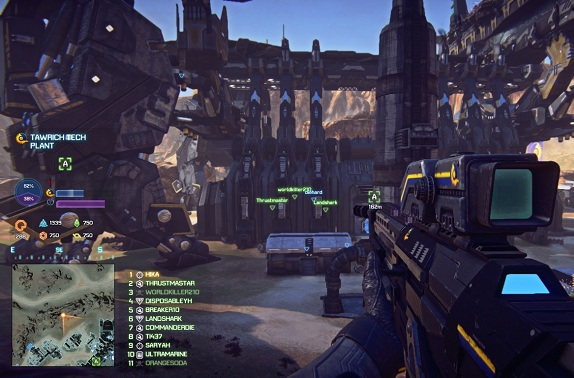
\includegraphics[width=\linewidth]{Figures/GameHUD.jpg}
	\decoRule
	\caption{A screenshot of the videogame \emph{Planetside 2}, showing its HUD. Locations of objectives and allies are indicated with triangles.}
	\label{fig:GameHUD}
\end{figure}

In order to apply a practical application to this, this project takes the visual HUD very popular in video games such as \emph{Planetside 2}, as seen in Figure~\ref{fig:GameHUD}, and reproduces it for use in the actual real world.  While there are many applications and ideas for a heads up display, this project is focused on locating and tracking certain points and other people within display. Hopefully, with further development and investment, this project expanded and improved upon for many applications. For example, keeping track of a person’s pulse while a surgeon is performing surgery or the marking of a very important target on a car’s windshield.

To keep track of a target for the AR application to find, tags are used to mark points, both of which are arbitrary and needed. The more tags available to use as points, the more accurate a reading would be. The tags use triangulation in order to locate and measure distance from the user, and to the point. A minimum of four tags are necessary to determine from the user to his destination in a 3D plane.

There are three main parts to this project: range finding, position calculation and augmented reality rendering. Range finding requires the use of the tags mentioned above to get the data fed to the device. Position calculation involves data processing from the tags within the device for use within the phone. Rendering will then take the data processed and put it on the screen.

[Insert image of cellphone screen with arrows and tag locations]

Range finding is done wirelessly with tags receiving packets of information to and from devices. The time it takes to receive broadcasted signals determine distances between sensors. These tags uses Ultra Wideband (UWB) to communicate between each other and the device together.

[insert image of tags here]
